\chapter{Potential Functions}
\label{chapter:potentialfunctions}

\FloatBarrier
\section{Introduction}

This section of the appendix covers the types of potential function and common choices of function used and details on how to use these in the potential fitting code.



\section{Functions}


%%%%%%%%%%%%%%%%%%%%%%%%%%%%%%%%%%%%%%%
% Ackland Embedding
%%%%%%%%%%%%%%%%%%%%%%%%%%%%%%%%%%%%%%%

\FloatBarrier
\subsection{Ackland Embedding}

\lstinputlisting[style=sFortran,caption={Ackland Embedding Fortran code}]{appendix/functions/pots_plots/fnc.ackland_embedding.f90}

\lstinputlisting[style=sOutputFile,caption={Ackland Embedding EAMPA input file}]{appendix/functions/pots_plots/ackland_embedding.pot}

\FloatBarrier
\begin{figure}[h]
  \begin{center}
    \includegraphics[width=0.7\linewidth]{appendix/functions/pots_plots/ackland_embedding.eps}
    \caption{Ackland Mendelev}
    \label{figure:functionsacklandmendelev}
  \end{center}
\end{figure}




%%%%%%%%%%%%%%%%%%%%%%%%%%%%%%%%%%%%%%%
% Buckingham
%%%%%%%%%%%%%%%%%%%%%%%%%%%%%%%%%%%%%%%

\FloatBarrier
\subsection{Buckingham}

\lstinputlisting[style=sFortran,caption={Buckingham Fortran code}]{appendix/functions/pots_plots/fnc.buckingham.f90}

\lstinputlisting[style=sOutputFile,caption={Buckingham EAMPA input file}]{appendix/functions/pots_plots/buckingham.pot}

\FloatBarrier
\begin{figure}[h]
  \begin{center}
    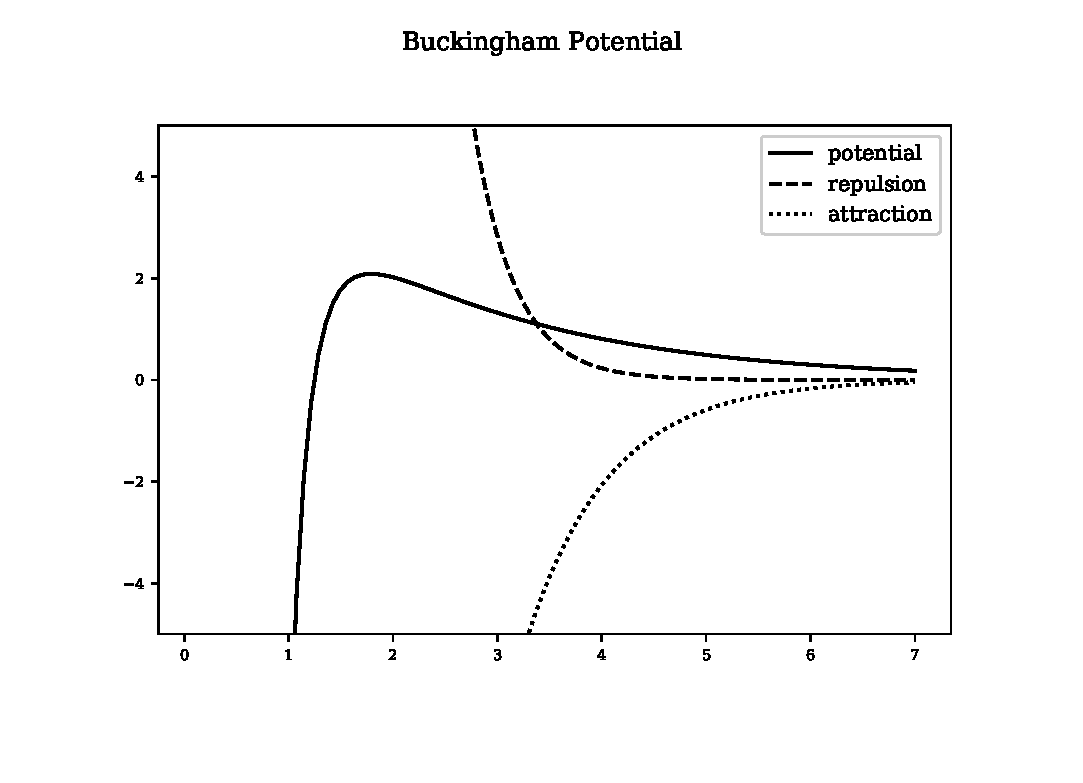
\includegraphics[width=0.7\linewidth]{appendix/functions/pots_plots/buckingham.eps}
    \caption{Buckingham}
    \label{figure:functionsbuckingham}
  \end{center}
\end{figure}




%%%%%%%%%%%%%%%%%%%%%%%%%%%%%%%%%%%%%%%
% Lennard Jones
%%%%%%%%%%%%%%%%%%%%%%%%%%%%%%%%%%%%%%%

\FloatBarrier
\subsection{Lennard Jones}

\lstinputlisting[style=sFortran,caption={Lennard Jones Fortran code}]{appendix/functions/pots_plots/fnc.lennard_jones.f90}

\lstinputlisting[style=sOutputFile,caption={Lennard Jones EAMPA input file}]{appendix/functions/pots_plots/lennard_jones.pot}

\FloatBarrier
\begin{figure}[h]
  \begin{center}
    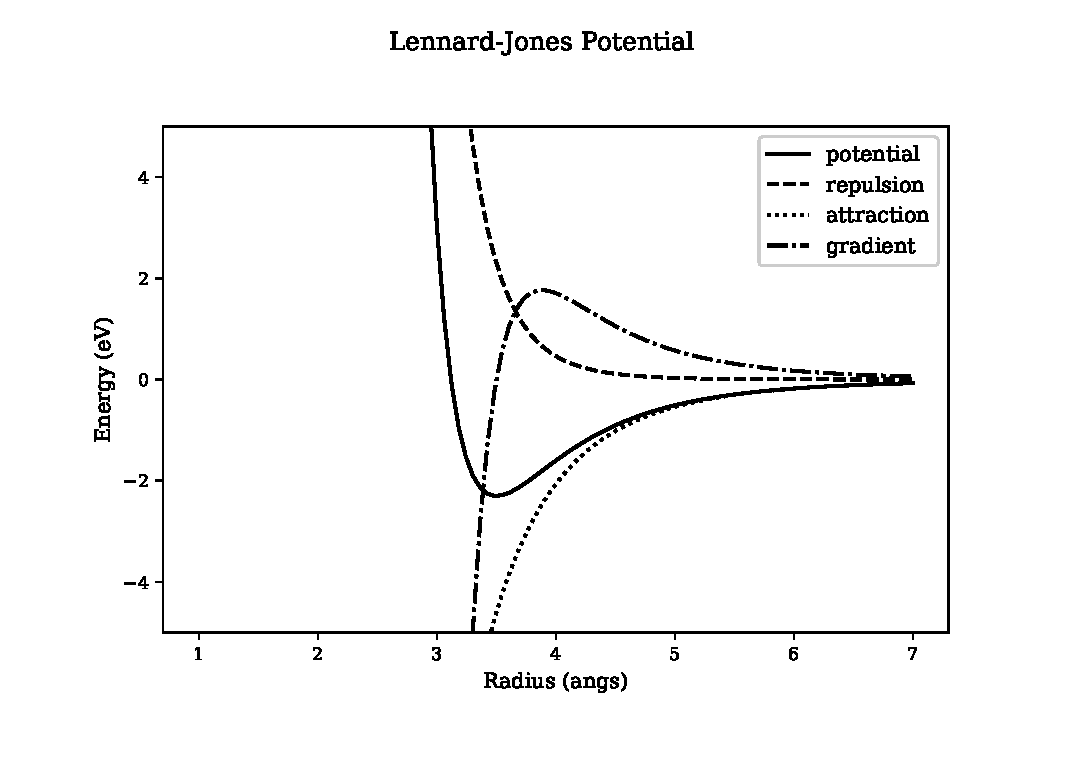
\includegraphics[width=0.7\linewidth]{appendix/functions/pots_plots/lennard_jones.eps}
    \caption{Lennard Jones}
    \label{figure:functionslennardjones}
  \end{center}
\end{figure}




%%%%%%%%%%%%%%%%%%%%%%%%%%%%%%%%%%%%%%%
% Mishin Density
%%%%%%%%%%%%%%%%%%%%%%%%%%%%%%%%%%%%%%%

\FloatBarrier
\subsection{Mishin Density}

\lstinputlisting[style=sFortran,caption={Mishin Density Fortran code}]{appendix/functions/pots_plots/fnc.mishin_density.f90}

\lstinputlisting[style=sOutputFile,caption={Mishin Density EAMPA input file}]{appendix/functions/pots_plots/mishin_density.pot}

\FloatBarrier
\begin{figure}[h]
  \begin{center}
    \includegraphics[width=0.7\linewidth]{appendix/functions/pots_plots/mishin_density.eps}
    \caption{Mishin Density}
    \label{figure:functionsmishindensity}
  \end{center}
\end{figure}




%%%%%%%%%%%%%%%%%%%%%%%%%%%%%%%%%%%%%%%
% Morse
%%%%%%%%%%%%%%%%%%%%%%%%%%%%%%%%%%%%%%%

\FloatBarrier
\subsection{Morse}

\lstinputlisting[style=sFortran,caption={Morse Fortran code}]{appendix/functions/pots_plots/fnc.morse.f90}

\lstinputlisting[style=sOutputFile,caption={Mishin Density EAMPA input file}]{appendix/functions/pots_plots/morse.pot}

\FloatBarrier
\begin{figure}[h]
  \begin{center}
    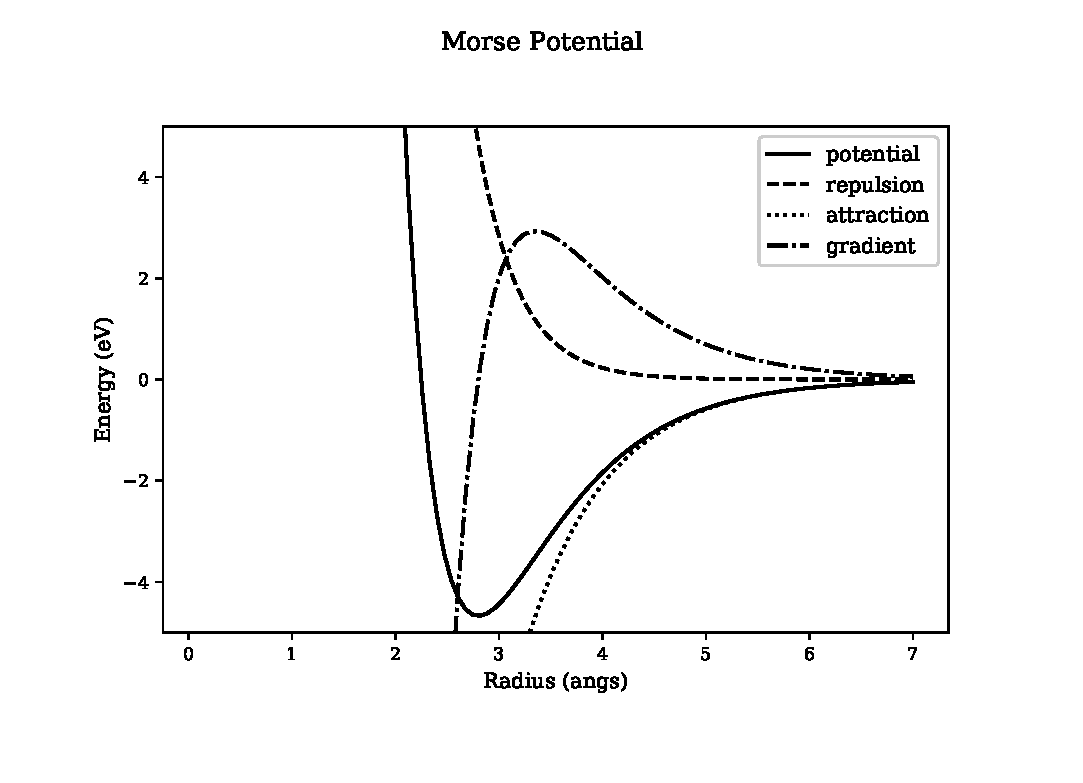
\includegraphics[width=0.7\linewidth]{appendix/functions/pots_plots/morse.eps}
    \caption{Morse}
    \label{figure:functionsmorse}
  \end{center}
\end{figure}




%%%%%%%%%%%%%%%%%%%%%%%%%%%%%%%%%%%%%%%
% Polynomial Embedding
%%%%%%%%%%%%%%%%%%%%%%%%%%%%%%%%%%%%%%%

\FloatBarrier
\subsection{Polynomial Embedding}

\lstinputlisting[style=sFortran,caption={Polynomial Embedding Fortran code}]{appendix/functions/pots_plots/fnc.polynomial_embedding.f90}

\lstinputlisting[style=sOutputFile,caption={Polynomial Embedding EAMPA input file}]{appendix/functions/pots_plots/polynomial_embedding.pot}

\FloatBarrier
\begin{figure}[h]
  \begin{center}
    \includegraphics[width=0.7\linewidth]{appendix/functions/pots_plots/polynomial_embedding.eps}
    \caption{Polynomial Embedding}
    \label{figure:functionspolynomialembedding}
  \end{center}
\end{figure}




%%%%%%%%%%%%%%%%%%%%%%%%%%%%%%%%%%%%%%%
% Spline
%%%%%%%%%%%%%%%%%%%%%%%%%%%%%%%%%%%%%%%

\FloatBarrier
\subsection{Spline}

\lstinputlisting[style=sFortran,caption={Spline Fortran code}]{appendix/functions/pots_plots/fnc.spline.f90}

\lstinputlisting[style=sOutputFile,caption={Spline EAMPA input file}]{appendix/functions/pots_plots/spline.pot}

\FloatBarrier
\begin{figure}[h]
  \begin{center}
    \includegraphics[width=0.7\linewidth]{appendix/functions/pots_plots/spline.eps}
    \caption{Spline}
    \label{figure:functionsspline}
  \end{center}
\end{figure}




%%%%%%%%%%%%%%%%%%%%%%%%%%%%%%%%%%%%%%%
% Slater 4s
%%%%%%%%%%%%%%%%%%%%%%%%%%%%%%%%%%%%%%%

\FloatBarrier
\subsection{Slater 4s}

\lstinputlisting[style=sFortran,caption={Slater 4s Fortran code}]{appendix/functions/pots_plots/fnc.slater_4s.f90}

\lstinputlisting[style=sOutputFile,caption={Slater 4s EAMPA input file}]{appendix/functions/pots_plots/slater_4s.pot}

\FloatBarrier
\begin{figure}[h]
  \begin{center}
    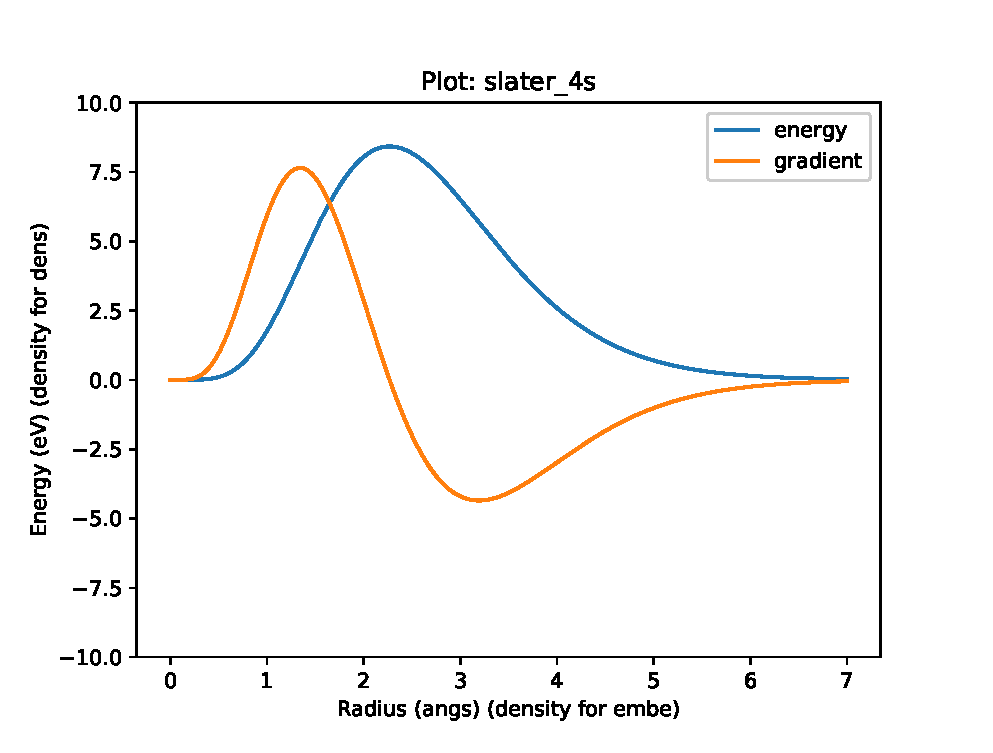
\includegraphics[width=0.7\linewidth]{appendix/functions/pots_plots/slater_4s.eps}
    \caption{Slater 4s}
    \label{figure:functionsslater4s}
  \end{center}
\end{figure}



%%%%%%%%%%%%%%%%%%%%%%%%%%%%%%%%%%%%%%%
% ZERO
%%%%%%%%%%%%%%%%%%%%%%%%%%%%%%%%%%%%%%%

\subsection{Zero}

\lstinputlisting[style=sFortran,caption={Zero Fortran code}]{appendix/functions/pots_plots/fnc.zero.f90}

\lstinputlisting[style=sOutputFile,caption={Zero EAMPA input file}]{appendix/functions/pots_plots/zero.pot}

\FloatBarrier
\begin{figure}[h]
  \begin{center}
    \includegraphics[width=0.7\linewidth]{appendix/functions/pots_plots/zero.eps}
    \caption{Zero}
    \label{figure:functionszero}
  \end{center}
\end{figure}






\FloatBarrier
\section{Splines}

\subsubsection{Polynomial Splines}
\label{section:backgroundpolynomialsplines}

The form of polynomial spline used in the literature is a sum of N cubic polynomials that, by way of the Heaviside step function and their form, cutoff neatly at the desired radius.  The cutoff radii are fixed and, during the fit of a potential, just the coefficients of each cubic spline are varied (eq. \ref{eq:cubicSpline}).

\begin{equation}
\begin{split}
V(r) = \sum_i^N a_i (r - r_i)^3 H(r_i - r) \\
\text{where } \\
H(x) = \left\{ \begin{matrix} 0 & x<0 \\  1 & x >= 0 \end{matrix} \right . 
\end{split}
\label{eq:cubicSpline}
\end{equation}

If a continuous second derivative is required the cubic spline may be replaced with a quintic spline (eq. \ref{eq:quinticSpline}).

\begin{equation}
\begin{split}
V(r) = \sum_i^N a_i (r - r_i)^5 H(r_i - r) \\
\end{split}
\label{eq:quinticSpline}
\end{equation}


\FloatBarrier
\subsubsection{Polynomial Knot to Knot Splines}

So far, analytic potentials have been discussed.  There are existing potentials that do not have an analytic form, but are tabulated data that have the properties that they are continuous and have a continuous first derivatives.  In attempting to fit or re-fit tabulated data, it would be problematic to adjust each data point individually given the number of data points and the requirement to have a continuous well behaved function with continuous first derivatives.

\begin{figure}[h]
  \begin{center}
    \includegraphics[scale=0.70]{chapters/interatomic_potential_fitting/plots_spline/spline.eps}
    \caption{Polynomial knot to knot spline}
    \label{fig:polynomialknots}
  \end{center}
\end{figure}

The tabulated function is divided into sections, and the start and end of each section forms the knot of the spline.  A polynomial may be splined between these knots, as shown in figure \ref{fig:polynomialknots}, but the order of polynomial will depend on the data available.  Immediately, the x and y positions are known: $x_a, x_b, f(x_a), f(x_b)$.  A first order polynomial has two unknowns, and so these unknowns may be calculated using linear algebra.

\begin{equation}
\begin{split}
c_0 + c_1 x_a = y_a \\
c_0 + c_1 x_b = y_b \\
\end{split}
\label{eq:cubicSpline}
\end{equation}

One of the requirements for the potential is to have a continuous first derivative, and this requires knowledge of the first derivative at each knot.  In the figure, the knots are shown as circles.  By taking several points near to each knot, shown as squares, the derivative at each knot may be calculated by interpolation.  This allows a third order polynomial to be used (eq. \ref{eq:eqSplineThreePoints}).

\begin{equation}
\begin{split}
      P_{1} = \left( x_A, f(x_A) \right) \\
      P_{2} = \left( x_A, f'(x_A) \right) \\
      P_{3} = \left( x_B, f(x_B) \right) \\
      P_{4} = \left( x_B, f'(x_B) \right)
\end{split}
\label{eq:eqSplineThreePoints}
\end{equation}

\begin{equation}
\begin{split}
c_0 + c_1 x_a + c_2 x_a^2 + c_3 x_a^3 = y_a \\
0 + c_1 + 2 c_2 x_a + 3 c_3 x_a^2 = y_a' \\
c_0 + c_1 x_b + c_2 x_b^2 + c_3 x_b^3 = y_b \\
0 + c_1 + 2 c_2 x_b + 3 c_3 x_b^2 = y_b' \\
\end{split}
\label{eq:cubicSpline}
\end{equation}

Rewriting as matrices:

\begin{equation}
\begin{split}
      \begin{bmatrix}
      1  &  x_a  &  {x_a}^2  &  {x_a}^3     \\
      0  &  1    &  2 x_a    &  3 {x_a}^2   \\
      1  &  x_b  &  {x_b}^2  &  {x_b}^3     \\
      0  &  1    &  2 x_b    &  3 {x_b}^2
      \end{bmatrix}
      \begin{bmatrix}
      c_0 \\
      c_1 \\ 
      c_2 \\ 
      c_3
      \end{bmatrix}
      = 
      \begin{bmatrix}
      f(x_a) \\
      f'(x_a) \\ 
      f(x_b) \\ 
      f'(x_b)
      \end{bmatrix}
\end{split}
\label{eq:eqSplineThreeMatrix}
\end{equation}

It is important for the function and its derivative to be continuous.  If it is also deemed necessary to have a continuous second derivative, a quintic spline may be used.  By interpolating and calculating the second order derivative at each knot, a 5th order polynomial may be splined between pairs of knots.  

This approach may be modified to spline functions of the form $\exp(p(r))$ between knots, and this is useful for splining between a \acrshort{zbl} or similar repulsive function at small r and a function of a different form at larger r.

\begin{equation}
\begin{split}
\text{where } \\
V(r) = \left\{ \begin{matrix} 
ZBL(r, q_1, q_2) & r<= r_a \\  
\exp(a+br+cr^2 + dr^3) & r_a < r < r_b \\ 
v(r) & r_b < r < r_{cut} \\ 
0 & r >= r_{cut} \\
\end{matrix} \right . 
\end{split}
\label{eq:zblCubicSpline}
\end{equation}

To spline the exponential the equations are set up in a similar way, but this time the system of equations are non-linear.

\begin{equation}
\begin{split}
\exp(c_0 + c_1 x_a + c_2 x_a^2 + c_3 x_a^3) = y_a \\
(c_1 + 2 c_2 x_a + 3 c_3 x_a^2)\exp(c_0 + c_1 x_a + c_2 x_a^2 + c_3 x_a^3) = y_a' \\
\exp(c_0 + c_1 x_b + c_2 x_b^2 + c_3 x_b^3) = y_b \\
(c_1 + 2 c_2 x_b + 3 c_3 x_b^2)\exp(c_0 + c_1 x_b + c_2 x_b^2 + c_3 x_b^3) = y_b' \\
\end{split}
\label{eq:cubicExpSpline}
\end{equation}

Newton-Gauss is used to solve this problem where initial parameters are set for the constants in the equation and varying until the function values and derivatives at point A and point B match the values being fitted to.


